\documentclass[a4paper,12pt]{article}

    \usepackage{graphicx}
    \usepackage{natbib}
    \usepackage{url}
    \usepackage[brazil]{babel}
    \usepackage[utf8]{inputenc}
    \usepackage[T1]{fontenc}

    %----------------------------------------------------------------------------------------
    %	DOCUMENT INFORMATION
    %----------------------------------------------------------------------------------------

    \title{Relatório do Trabalho Prático 3} % Title
    % \author{Ramon \textsc{Melo}} % Author name
    % \date{\today} % Date for the report

    \begin{document}

        \maketitle % Insert the title, author and date

        \begin{center}
            \begin{tabular}{l r}
                % Data: & \today \\ % Date the experiment was performed
                Aluno: & Ramon Melo \\ % Partner names
                Professor: & Daniel Figueiredo \\ % Instructor/supervisor
                \multicolumn{2}{r}{\url{https://github.com/ramonduarte/sd3}}
            \end{tabular}
        \end{center}

         %----------------------------------------------------------------------------------------
        %	SECTION 1
        %----------------------------------------------------------------------------------------
        
        \section{Objetivo}
        
            Construir um sistema distribuído cujo mecanismo de ordenação total de eventos seja baseado no algoritmo \emph{Totally Ordered Multicast}, utilizando o relógio lógico de Lamport como ordenador.
            
        %----------------------------------------------------------------------------------------
        %	SECTION 2
        %----------------------------------------------------------------------------------------
        
        \section{Decisões de Projeto}

            \emph{O código utilizado para este trabalho, bem como os logs dos estudos de caso, as imagens, o relatório e a apresentação, estão disponíveis publicamente no caminho \url{https://github.com/ramonduarte/sd3}}.
        
            \emph{}Ao contrário dos trabalhos anteriores, a ordenação total de eventos distribuídos ocorre numa camada de abstração significativamente acima do hardware, de forma que implementações de baixo nível e acesso direto ao metal não compõem mais o conjunto de ferramentas desejável ao desenvolvimento da aplicação.
            Pelo contrário, bibliotecas de \emph{sockets}, processos e \emph{user-level threads} estão disponíveis em praticamente todas as linguagens de programação.
            Desta forma, deseja-se do ecossistema características como o suporte a construtos de programação orientada a objetos, tais como herança e polimorfismo; legibilidade do código; e agnosticismo em relação ao sistema operacional.
            
            A linguagem escolhida para este trabalho foi Python 3.5, edição que é nativa à maioria esmagadora de sistemas operacionais baseados no padrão POSIX.
            Em especial, esta versão é significativamente mais eficiente que as baseadas em Python 2 - mais tradicionais - e traz nativamente bibliotecas como a \texttt{multiprocessing} - \emph{user-level threads} em concorrência, uma das poucas implementações que suporta o ecossistema Windows (\cite{WEBSITE:8}).
            
            Dada a natureza dos requisitos, que exige estruturas de dados razoavelmente similares mas autônomas, e ao prazo de entrega, que forçou a realização de \emph{sprints} bastante curtos (em média, dois por semana), o paradigma de orientação a objetos foi uma escolha natural.

            Conforme sugestão do enunciado, a comunicação interprocessual foi mantida através de \emph{sockets} TCP, o que, na prática, implica a premissa de que a rede física subposta é confiável, ou seja, mensagens não são perdidas (e, portanto, não precisam ser reenviadas) e chegam convenientemente de acordo com a ordem em que foram enviadas (\cite{KuroseRoss2007}).
            Esta premissa pode ser considerada verdadeira para \emph{sockets} locais, que não dependem de canais externos ao sistema operacional para completarem o percurso.
            Por esta razão, os estudos de caso foram realizados no mesmo computador, onde tal presunção pode ser verificada e mensurada.

            É importante mencionar que, devido à especificação do trabalho, ferramentas de altíssimo nível de abstração foram propositalmente evitadas, visto que mascarariam funcionalidades requeridas pelo enunciado.
            Ainda assim, é relevante mencioná-las, para fins de completude desta seção.
            O módulo \texttt{socketserver} gerencia silenciosamente falhas de conexão em \emph{sockets}, e seria a principal escolha se não houvesse especificada a necessidade de coordenar manualmente os \emph{sockets}.
            Caso não houvesse a necessidade de utilizar uma \emph{thread} cliente e outra servidora, o módulo \texttt{asyncio} seria uma escolha mais intuitiva.
            Se esta fosse uma aplicação comercial, muitas das funcionalidades já estariam implementadas no framework \emph{Twisted}, direcionado a arquiteturas orientadas a eventos, como é o caso aqui (\cite{WEBSITE:11}).

            Embora a linguagem preveja implementação agnóstica em relação aos sistemas operacionais, esta aplicação foi desenvolvida sob o sistema operacional Ubuntu 14.04 LTS 64-bit, onde a implementação é determinística (\cite{WEBSITE:8}).
            Em especial, versões antigas de sistemas Windows podem exibir condições de corrida não-previsíveis.

            O programa foi projetado para ser executado por um interpretador no modo otimizado (\texttt{python -O main.py [args]}).
            Embora o modo não-otimizado produza o mesmo resultado para fins práticos, há diversos gatilhos de depuração (\texttt{if \_\_debug\_\_}) que serão ativados.
            A avaliação pode se tornar cansativa ou tediosa devido à verbosidade das diretivas de depuração.

        %----------------------------------------------------------------------------------------
        %	SECTION 3
        %----------------------------------------------------------------------------------------
        
        \section{Implementação}
        
        Há cinco classes que serviram de fundação para o trabalho.
        O diagrama de classes está representado graficamente na Figura 1.

        \begin{figure}[h]
            \begin{center}
                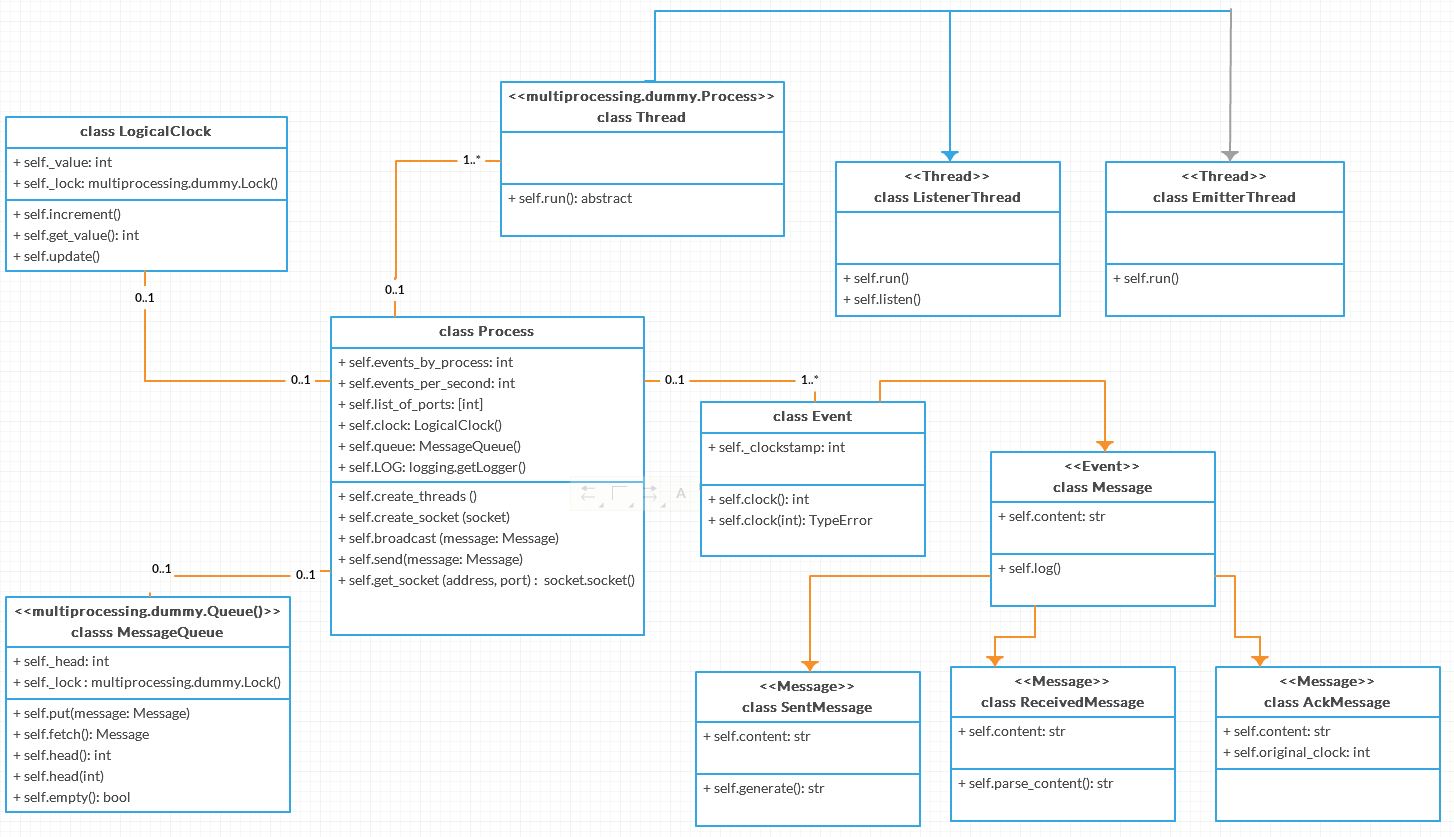
\includegraphics[width=1\textwidth]{class-diagram}
                \caption{Diagrama de Classes da implementação.}
            \end{center}
        \end{figure}

        A classe \texttt{Process} encapsula funcionalidades dos módulos \texttt{socket} (\cite{WEBSITE:7}) e \texttt{multiprocessing}.
        É importante observar que este último expõe a mesma \emph{API} tanto para processos, quanto para \emph{threads}.
        Devido aos requerimentos do enunciado, foi utilizado somente o \emph{namespace} \texttt{dummy}, que inicia \emph{user-level threads} dentro do mesmo processo e permite o compartilhamento implícito de memória entre elas.
        Para cada \texttt{Process}, é aberto um total de 3 \emph{threads}: uma cliente, uma servidora e uma principal, responsável pelo gerenciamento dos recursos do processo.
        O encerramento desta última automaticamente interrompe as demais e ativa a coleta de lixo e desalocação de recursos, incluindo os \emph{sockets} previamente alocados.
        
        O autor observou que, a despeito disto, eles permanecem abertos e ocupando o endereço por algum tempo, presumidamente por opção do sistema operacional (\cite{WEBSITE:9}).
        Caso isto ocorra, o programa acionará uma exceção \texttt{ConnectionRefusedError} e encerrará logo em seguida.
        Falhas capturadas pelo interpretador Python, incluindo o comando \texttt{CTRL+C}, provocarão, como reação, a tentativa de fechar todos os \emph{sockets} antes de encerrar a execução.
        Falhas que escapam ao contexto do interpretador (como o sinal \texttt{SIGKILL}) provocarão o encerramento abrupto, caso em que \texttt{ConnectionRefusedError}s são mais prováveis de ocorrer. 

        A classe \texttt{Thread} concentra os métodos executados concorrentemente.
        Em especial, o método \texttt{run()} foi construído desde o princípio de forma limitada ao padrão \emph{thread-safe}.
        Herdam desta classe \texttt{ListenerThread} (orientada a serviços de servidor) e \texttt{EmitterThread} (orientada a serviços de cliente).

        Os objetos que representam os eventos são derivados da classe \texttt{Event}.
        Particularmente, os que representam as mensagens derivam da classe \texttt{Message}.
        São eles: \texttt{SentMessage} (enviada pelo processo que a criou), \texttt{ReceivedMessage} (recebida pelo processo que a criou) e \texttt{AckMessage} (confirmação a ser enviada pelo processo que a criou).
        As mensagens são as responsáveis pela execução, visto que representam os eventos na abstração do mecanismo \emph{Totally Ordered Multicast} enunciada a este trabalho.
        Portanto, é a classe \texttt{ReceivedMessage} a responsável por gravar pertinentemente as mensagens no disco uma vez que estejam aptas.

        O relógio lógico de Lamport é representado pela classe \texttt{LogicalClock}, que encapsula cadeados (\emph{locks}) para a manutenção do caráter \emph{thread-safe} do método \texttt{Thread.run()}.

        Por fim, as mensagens que aguardam execução são armazenadas num objeto \texttt{MessageQueue}, que encapsula uma fila do tipo \emph{FIFO} (\emph{First In, First Out}, "fila indiana") e cadeados para seu acesso concorrente.

        Todos os objetos são pertencentes ao objeto \texttt{Process} que coordena a execução local do programa.
        Isto porque, para garantir o acesso implícito à memória compartilhada, o módulo \texttt{multiprocessing} exige que as estruturas de dados sejam referenciadas pela abstração do processo (e não pela das \emph{threads}).

        A escrita no disco é gerenciada pelo modo \texttt{logging}, que grava num arquivo sugerido pelo próprio usuário como comando.

        Os argumentos passados ao arquivo \texttt{main.py} incluem o nome do arquivo do log onde os eventos serão gravados, o número $n$ de mensagens enviadas por processo, a taxa $\lambda$ de emissão de mensagens por segundo e o total $p$ de processos abertos simultaneamente.

            
        %----------------------------------------------------------------------------------------
        %	SECTION 4
        %----------------------------------------------------------------------------------------
        
        \section{Estudos de Caso}
        
        Os estudos de caso foram executados para as combinações dos valores $n \in \{1, 2, 4, 8\}$, $\lambda \in \{100, 1000, 10000\}$ e $p \in \{1, 2, 10\}$.
        Foram usadas portas de numeração entre 8000 e 8007, por serem comumente livres na maioria dos sistemas.
        Os valores podem ser conferidos na Tabela 1.
        Os logs estão disponíveis no repositório onde o trabalho foi hospedado, na pasta \texttt{logs/}.

        A análise dos tempos corrobora a premissa de rede confiável, sobretudo se se considerar que os testes foram conduzidos em \texttt{localhost}.
        A complexidade da execução é trivialmente verificável como $O(n)$ e $O(\lambda)$.
        O número de processos teve impacto desprezível sobre o tempo total de execução.

        Um olhar mais perspicaz sobre os logs, porém, revela que houve um número significativo de processos interrompidos antes do tempo.
        A maioria das falhas críticas parece apontar para a perda de conexão do \emph{socket}, haja vista que o interpretador Python levanta a exceção \texttt{BrokenPipeError} nestas condições.
        Há, contudo, um conjunto de exceções que não foram capturadas, provocando o encerramento precoce dos processos.
        Como a falha só foi detectada às vésperas do prazo, não houve tempo hábil de depurá-la.
        A justificativa para tanto é o fato de só ser possível notar tal aspecto lendo os logs até o fim, que são arquivos cuja extensão desafia os limites da janela de atenção do cérebro humano.

        \begin{table}[]
            \centering
            \begin{tabular}{rrrll}
                \hline
                \multicolumn{1}{l}{$p$}   & \multicolumn{1}{l}{$\lambda$} & \multicolumn{1}{l}{tempo (s)}  \\ \hline
                2                       & 1                             & 28.52374                       \\
                2                       & 2                             & 12.420049                      \\
                2                       & 10                            & 2.959135                       \\
                4                       & 1                             & 59.568429                      \\
                4                       & 2                             & 29.813078                      \\
                4                       & 10                            & 5.086868                       \\
                8                       & 1                             & 109.699103                     \\
                8                       & 2                             & 55.250551                      \\ 
                8                       & 10                            & 10.990417                      \\ \hline
            \end{tabular}
            \begin{tabular}{rrrll}
                \hline
                \multicolumn{1}{l}{$p$} & \multicolumn{1}{l}{$\lambda$} & \multicolumn{1}{l}{tempo (s)} \\ \hline
                2                       & 1                           & 286.246658                    \\
                2                       & 2                           & 148.901997                    \\
                2                       & 10                          & 29.346077                     \\
                4                       & 1                           & 585.1391                      \\
                4                       & 2                           & 296.462348                    \\
                4                       & 10                          & 59.496107                     \\
                8                       & 1                           & 1152.87353                    \\
                8                       & 2                           & 585.239865                    \\
                8                       & 10                          & 113.358163                    \\ \hline
            \end{tabular}
            \begin{tabular}{rrrll}
                \hline
                \multicolumn{1}{l}{$p$} & \multicolumn{1}{l}{$\lambda$} & \multicolumn{1}{l}{tempo (s)} \\ \hline
                2                       & 1                             & 2998.55037                    \\
                2                       & 2                             & 1494.091501                   \\
                2                       & 10                            & 297.763825                    \\
                4                       & 1                             & 5883.879098                   \\
                4                       & 2                             & 2979.343469                   \\
                4                       & 10                            & 600.332818                    \\
                8                       & 1                             & 11834.078567                  \\
                8                       & 2                             & 5929.261745                   \\
                8                       & 10                            & 1182.840992                   \\\hline
            \end{tabular}
            \caption{(a) $n = 100$; (b) $n = 1000$; (c) $n = 10000$.}
            \label{my-label}
        \end{table}

        
        %----------------------------------------------------------------------------------------
        %	SECTION 5
        %----------------------------------------------------------------------------------------
        
        \section{Considerações Finais}
        
        Apesar de simples em essência, a implementação deste mecanismo foi cercada de desafios teóricos e práticos.
        O tempo total de desenvolvimento foi de 116 horas, divididas em 3 semanas. 
        
        A principal dificuldade, do ponto de vista teórico, foi a construção do diagrama de classes para o projeto.
        As escolhas que pareciam mais prováveis para uma comunicação entre dois processos provaram-se desastrosas quando expandidas.

        Do ponto de vista prático, o principal desafio foi gerenciar a integridade dos \emph{sockets}.
        A biblioteca nativa do Python 3.5 não possui um método confiável de checagem de integridade.
        De fato, a recomendação oficial é, justamente, que se tente enviar mensagens quando desejado e que se capture a exceção \texttt{BrokenPipeError} quando levantada.

        Ainda assim, o autor acredita que o projeto promoveu uma revisão abrangente e profunda da ordenação total de eventos em sistemas distribuídos.
        De fato, se refeito do princípio, haveria um esforço maior na etapa de manutenção da integridade dos \emph{sockets}, visto que são, de longe, o maior gargalo desta implementação.


        %----------------------------------------------------------------------------------------
        %	BIBLIOGRAPHY
        %----------------------------------------------------------------------------------------
        
        \bibliographystyle{apalike}
        \bibliography{sd3_report}
        
        %----------------------------------------------------------------------------------------


    \end{document}